% !TEX encoding = UTF-8 Unicode
%%
%%		XX_名前_日付.{tex,pdf}
%%		XX, 名前, 日付は naming rule に従う
%%
\documentclass[11pt,a4paper]{jsarticle}

%% ページ設定のパラメータは変更しない
\usepackage[top=72pt,bottom=60pt,left=40pt,right=40pt]{geometry}
\setlength{\topmargin}{-38pt}
\setlength{\headheight}{18pt}
\setlength{\headsep}{20pt}
\setlength{\footskip}{38pt}
\setlength{\topskip}{0pt}
%%

%% 共通フォーマット
\usepackage{fancyhdr}
\rhead{\stdid, \sirname}
\cfoot{}
\rfoot{\thepage}
\renewcommand{\footrulewidth}{\headrulewidth}
\pagestyle{fancy}

\usepackage{subfig}
\usepackage{layout}

%% \title{maketitleは使わない}
%% \author{}
%% \date{}

%% 自分の使うパッケージ
\usepackage{amsmath,amssymb}
\usepackage{bm}
\usepackage[dvipdfmx]{graphicx}
\usepackage{ascmac}
\usepackage{indentfirst}
\graphicspath{{./images/}}

%% 個人設定、日付設定
\lfoot{2019年 9月23日}		%% 日付
\def\stdid{18T0006}		%% 学生証番号
\def\sirname{小室}		%% 姓
\def\firstname{光広}		%% 名


\begin{document}
%% \maketitle			%% maketitle は使わない

\noindent
\textbf{\large 進捗レポート (\stdid, \sirname\ \firstname)}		%%  固定

%%
\section*{今週の進捗サマリ}			%% 固定

\begin{itemize}
  \item シングルエージェントでのextended実験
  \item マルチエージェント化実装
\end{itemize}

%%
\section{進捗詳細}					%% 固定
\subsection{シングルエージェントでのextended実験}
2019年9月10日に行われたゼミの際にご指摘いただいた結果が悪かったモデルについて追加で
400episode学習を進める追加実験を行った.結果,pongの点数としては21-6でモデルの負けであるが,
1点追加で点数を上げることができた.なお,本追加実験ではRandom値を固定していないモデルである.\par
次にシングルエージェントでのSeedを固定した結果について示す.


\subsection{マルチエージェント化実装}
シングルエージェントで使用したPong用のサンプルコードをSeedFixedなマルチエージェントコードに書き換える作業を行っている.
当初の案ではマルチエージェント化手法としてパイプライン的に行う\textit{Sync(仮称)}とマルチスレッド的に行う\textit{Async(仮称)}を
想定していた.
\begin{figure}[htbp]
  \begin{center}
    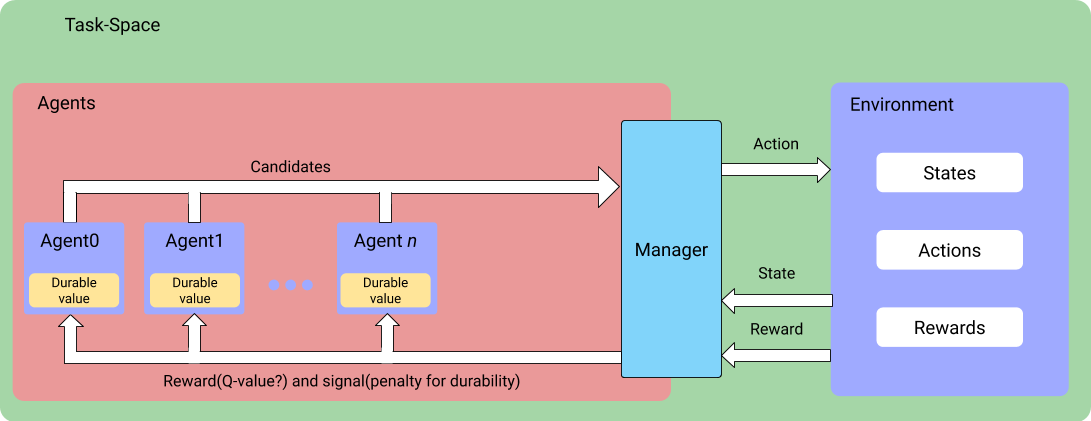
\includegraphics[width=14cm]{fig1.png}
    \caption{Sync(仮称)モデル}
  \end{center}
  \label{fig1}
\end{figure}
ここから大きく変わることは無いが,Syncモデルをメインに実装しており,実装上SyncモデルにおけるManager及びEnvironmentの関係について
変更する必要が出てきた.変更点を以下に示す.

\begin{itemize}
  \item 各Agent0からAgent nまでそれぞれにEnvironmentが必要
  \item Managerとしていたものを\texttt{core\_agent}として,図1のEnvironmentを\texttt{core\_environment}とする
\end{itemize}

各AgentからActionを候補として出す際,どうしてもEnvironmentのStepが進んでしまうため,正しい学習とは言えなくなってしまう可能性がある,
つまりAgentのAction n個分だけ変化したEnvironmentをManagerが扱う事となってしまう.この場合,FrameSkipに類似する現象と考えられるため,
精度低下が考えられる.次にManagerをAgent化することについて,Managerの実装を考えたとき,各AgentからBestなActionを起こすAgentを選び,
そのActionを実際にManagerからEnvironmentにやってほしいので,実装上Managerを\texttt{core\_agent}として扱うこととした.\par
これらを踏まえ,現在Agent class及びEnvironment class, Train stepの関数までは実装できているが,学習ループ中にRuntimeErrorで動作が
停止することを確認しており,修正中である.best Agentを耐久値0以下のAgentにDeepコピーすることでAgentsの淘汰を行っているが,それが一因と
なっている可能性も考えられ,どこを修正すればいいのか手探りな状態であるため,時間を要すると考える.早期の解決を目指したい.

\section{今後の予定}
前述の通り,大まかな実装が完了したものの,Agentの淘汰等細かい部分でバグが発生しているため,実験まで到達していない状況である.
9月は残り1週となり非常に厳しい状況だが,今月中の実装を目指したい.また,次週ゼミまでにSeedFixedなシングルAgentのサンプルコードでの実験
を行いたい.

\end{document}

